\documentclass[../../main.tex]{subfiles}

\begin{document}

\chapter{Kriptografi Kunci-Publik: Algoritma Knapsack}
\label{chap:knapsack}

\begin{learningoutcome}
Setelah mempelajari bab ini, mahasiswa diharapkan mampu:
\begin{itemize}
    \item Menjelaskan konsep dasar persoalan \textit{Knapsack Problem} dan kaitannya dengan kriptografi kunci-publik (Sub-CPMK 1.3).
    \item Membedakan secara jelas antara barisan \textit{superincreasing} dan barisan \textit{non-superincreasing} (Sub-CPMK 1.3).
    \item Menerapkan prosedur enkripsi dan dekripsi pada sistem kriptografi Merkle-Hellman (Sub-CPMK 1.3).
    \item Menganalisis proses transformasi kunci privat menjadi kunci publik dalam sistem Knapsack (Sub-CPMK 1.3).
    \item Mengevaluasi keamanan algoritma Knapsack dan memahami alasan mengapa sistem ini tidak lagi dianggap aman (Sub-CPMK 1.3).
\end{itemize}
\end{learningoutcome}

\subfile{section-01}
\subfile{section-02}
\subfile{section-03}
\subfile{section-04}
\section{Contoh Terhitung}
\label{sec:contoh-knapsack}

Contoh-contoh pada bagian ini disusun mengikuti alur perancangan sistem
Merkle--Hellman, dari persoalan yang paling dasar sampai prosedur lengkapnya.
Contoh pertama memperlihatkan mengapa \textit{knapsack} biasa tidak dapat
didekripsi; contoh kedua memperlihatkan bagaimana barisan superincreasing
menyelesaikan persoalan itu; contoh ketiga memperlihatkan bahwa kemudahan
tersebut justru harus disembunyikan; dan dua contoh terakhir menjalankan
seluruh prosedur dari pembangkitan kunci sampai pemulihan plainteks. Setiap
angka di bawah ini telah diverifikasi dengan program pada bagian praktikum di
akhir bab ini.

\begin{example}[Knapsack biasa: mudah dienkripsi, sulit didekripsi]
\label{ex:knapsack-dasar}
Misalkan barisan bobot yang disepakati adalah
\[ W = \{1, 5, 6, 11, 14, 20\} . \]
Barisan ini \emph{bukan} barisan superincreasing, sebab $6 > 1 + 5 = 6$ gagal
dan $11 > 1 + 5 + 6 = 12$ juga gagal
(Subbagian~\ref{subsec:greedy-knapsack}). Karena itu algoritma \textit{greedy}
tidak dapat dipakai di sini.

Pesan yang hendak dikirim adalah rangkaian biner
\[ \code{111001010110000000011000} , \]
yang dipecah menjadi blok-blok sepanjang enam bit. Karena $2^{6} = 64$ dan
seluruh bobot berjumlah $57$, setiap blok dapat diwakili. Hasil enkripsinya
diperlihatkan pada Tabel~\ref{tab:knapsack-dasar}.

\begin{table}[htbp]
    \centering
    \begin{tabular}{@{}l c r@{}}
    \toprule
    \textbf{Blok} & \textbf{Bobot yang dipilih} & \textbf{Kriptogram} \\
    \midrule
    \code{111001} & $1 + 5 + 6 + 20$      & $32$ \\
    \code{010110} & $5 + 11 + 14$         & $30$ \\
    \code{000000} & ---                   & $0$ \\
    \code{011000} & $5 + 6$               & $11$ \\
    \bottomrule
    \end{tabular}
    \caption{Enkripsi empat blok pesan dengan barisan
    $W = \{1, 5, 6, 11, 14, 20\}$. Setiap blok menjadi sebuah bilangan
    tunggal}
    \label{tab:knapsack-dasar}
\end{table}

Jadi kriptogramnya adalah barisan bilangan $(32, 30, 0, 11)$.
Sekarang perhatikan pihak penerima. Bila ia tidak mengetahui $W$, ia hanya
memegang bilangan $32$ dan harus menebak himpunan bagian mana yang
jumlahnya $32$. Dengan enam elemen ada $2^{6} = 64$ kemungkinan, dan
menelusurinya masih mungkin. Namun untuk $n = 250$ kemungkinannya menjadi
$2^{250}$, dan tidak ada cara yang diketahui untuk menghindari penelusuran itu
secara menyeluruh --- kecuali bila barisannya superincreasing.

Perlu diperhatikan bahwa blok terakhir, \code{011000}, menghasilkan kriptogram
$11$ yang \emph{sama} dengan elemen $w_4 = 11$ itu sendiri. Keadaan semacam
itu adalah petunjuk yang tidak diinginkan: sebuah kriptogram dapat kebetulan
sama dengan salah satu elemen barisan bobot, dan penyadap dapat memanfaatkan
kebetulan itu. Pada $n$ yang besar, kebetulan seperti itu terlalu sering
terjadi untuk diabaikan.

\par\vspace{2pt}{\footnotesize\itshape Catatan: berkas sumber menuliskan
plainteksnya sebagai \code{1110010101100000000011000} yang panjangnya 25 bit.
Rangkaian itu tidak konsisten dengan keempat blok pada tabel di atas; rangkaian
yang benar adalah \code{111001010110000000011000} yang panjangnya 24 bit.\par}
\end{example}

\begin{example}[Dekripsi \textit{greedy} pada barisan superincreasing]
\label{ex:greedy-superincreasing}
Sekarang dipakai barisan superincreasing
\[ W = \{2, 3, 6, 13, 27, 52\} , \qquad \sum_{i=1}^{6} w_i = 103 . \]
Barisan ini memenuhi Persamaan~\eqref{eq:superincreasing}: $3 > 2$,
$6 > 2+3 = 5$, $13 > 2+3+6 = 11$, $27 > 2+3+6+13 = 24$, dan
$52 > 2+3+6+13+27 = 51$.

Diberikan kriptogram $M = 70$. Algoritma \textit{greedy} berjalan dari elemen
terbesar ke terkecil, dan setiap langkahnya diperlihatkan pada
Tabel~\ref{tab:greedy-70}.

\begin{table}[htbp]
    \centering
    \begin{tabular}{@{}c c c c@{}}
    \toprule
    \textbf{Bobot} & \textbf{Sisa $M$} & \textbf{Perbandingan} &
    \textbf{Bit} \\
    \midrule
    $52$ & $70$ & $52 \le 70$  & $b_6 = 1$, sisa menjadi $18$ \\
    $27$ & $18$ & $27 > 18$    & $b_5 = 0$ \\
    $13$ & $18$ & $13 \le 18$  & $b_4 = 1$, sisa menjadi $5$ \\
    $6$  & $5$  & $6 > 5$      & $b_3 = 0$ \\
    $3$  & $5$  & $3 \le 5$    & $b_2 = 1$, sisa menjadi $2$ \\
    $2$  & $2$  & $2 \le 2$    & $b_1 = 1$, sisa menjadi $0$ \\
    \bottomrule
    \end{tabular}
    \caption{Langkah demi langkah algoritma \textit{greedy} untuk $M = 70$}
    \label{tab:greedy-70}
\end{table}

Karena sisa akhirnya nol, solusinya sah, dan bitnya terbaca dari belakang:
\[ (b_1, b_2, b_3, b_4, b_5, b_6) = (1, 1, 0, 1, 0, 1) = \code{110101} . \]
Pemeriksaannya: $2 + 3 + 13 + 52 = 70$. Algoritma ini hanya memerlukan enam
perbandingan --- linier terhadap panjang barisan, bukan eksponensial.

Perhatikan langkah terakhir, ketika $M = 2$ dan bobot yang tersisa adalah
$w_1 = 2$. Karena $2 \le 2$, bitnya bernilai $1$. Berkas sumber menuliskan
langkah ini sebagai $2 - 2 = 0$ dengan $b_1 = 0$ --- jelas tidak konsisten,
sebab bila $b_1 = 0$ maka sisanya tetap $2$ dan bukan $0$. Bit yang benar
adalah $b_1 = 1$, sebagaimana ditegaskan oleh jawaban akhir \code{110101} yang
tercantum pada berkas yang sama.
\end{example}

\begin{example}[Pembangkitan kunci publik]
\label{ex:mh-kunci-105}
Barisan $W = \{2, 3, 6, 13, 27, 52\}$ terlalu mudah dipecahkan untuk dipakai
langsung (Contoh~\ref{ex:greedy-superincreasing}). Karena itu ia dijadikan
kunci privat, dan barisan publiknya dibangkitkan dengan
Persamaan~\eqref{eq:mh-kunci}. Pilih
\[ m = 105 \quad (\text{lebih besar daripada } 103), \qquad n = 31 , \]
dengan $\text{PBB}(31, 105) = 1$. Barisan publiknya:

\begin{table}[htbp]
    \centering
    \begin{tabular}{@{}c c c c@{}}
    \toprule
    $i$ & $w_i$ & $w_i \cdot n$ & $w'_i = (w_i \cdot 31) \bmod 105$ \\
    \midrule
    $1$ & $2$  & $62$  & $62$ \\
    $2$ & $3$  & $93$  & $93$ \\
    $3$ & $6$  & $186$ & $81$ \\
    $4$ & $13$ & $403$ & $88$ \\
    $5$ & $27$ & $837$ & $102$ \\
    $6$ & $52$ & $1612$ & $37$ \\
    \bottomrule
    \end{tabular}
    \caption{Pembangkitan kunci publik dari
    $W = \{2, 3, 6, 13, 27, 52\}$ dengan $m = 105$ dan $n = 31$}
    \label{tab:mh-kunci-105}
\end{table}

Jadi $W_{pub} = \{62, 93, 81, 88, 102, 37\}$. Perhatikan bahwa barisan ini
sudah tidak superincreasing lagi: $81 < 62 + 93$, dan $37$ yang tadinya
elemen terbesar justru menjadi paling kecil. Sifat mudahnya benar-benar
lenyap dari pandangan.

Karena $\text{PBB}(31, 105) = 1$, inversnya ada. Dari
$31 \cdot 61 = 1891 = 18 \cdot 105 + 1$ diperoleh
\[ n^{-1} = 31^{-1} \bmod 105 = 61 . \]
Nilai inilah yang dipegang penerima, dan nilainya menjadi rahasia.
\end{example}

\begin{example}[Enkripsi dan dekripsi dengan kunci publik buatan sendiri]
\label{ex:mh-105}
Melanjutkan Contoh~\ref{ex:mh-kunci-105}, pesan yang dikirim adalah
\[ \code{011000110101101110} , \]
yang dipecah menjadi tiga blok sepanjang enam bit:
\code{011000}, \code{110101}, dan \code{101110}.

\textbf{Enkripsi.} Pengirim memakai $W_{pub}$ dan
Persamaan~\eqref{eq:mh-enkripsi}:
\begin{align*}
\code{011000} &\to 93 + 81 = 174, \\
\code{110101} &\to 62 + 93 + 88 + 37 = 280, \\
\code{101110} &\to 62 + 81 + 88 + 102 = 333 .
\end{align*}
Kriptogram yang dikirim adalah $(174, 280, 333)$. Perhatikan bahwa $280$ dan
$333$ keduanya melampaui modulus $m = 105$. Itu memang tidak menjadi masalah,
sebab dekripsi hanya memakai nilai $C \bmod m$
(Subbagian~\ref{subsec:bukti-knapsack}).

\textbf{Dekripsi.} Penerima mengalikan tiap kriptogram dengan $n^{-1} = 61$
modulo $105$ menurut Persamaan~\eqref{eq:mh-dekripsi}:

\begin{table}[htbp]
    \centering
    \begin{tabular}{@{}r r l@{}}
    \toprule
    $C$ & $C' = (C \cdot 61) \bmod 105$ & \textbf{Hasil \textit{greedy}} \\
    \midrule
    $174$ & $9$  & $6 + 3 = 9$ $\to$ \code{011000} \\
    $280$ & $70$ & $52 + 13 + 3 + 2 = 70$ $\to$ \code{110101} \\
    $333$ & $48$ & $27 + 13 + 6 + 2 = 48$ $\to$ \code{101110} \\
    \bottomrule
    \end{tabular}
    \caption{Dekripsi ketiga blok. Nilai $C'$ jatuh kembali ke dalam barisan
    superincreasing, sehingga algoritma \textit{greedy} dapat dipakai}
    \label{tab:mh-105-dekripsi}
\end{table}

Ketiga blok pulih tepat seperti semula, sehingga plainteksnya kembali menjadi
\code{011000110101101110}.

Contoh ini memperlihatkan inti sistem Merkle--Hellman dalam bentuk yang paling
telanjang. Pengirim tidak pernah menyentuh barisan superincreasing; ia hanya
menjumlahkan elemen-elemen publik. Penerima juga tidak pernah memecahkan
\textit{knapsack} publik; ia cukup mengalikan kriptogram dengan $61$ modulo
$105$, dan persoalannya seketika kembali menjadi mudah.

\par\vspace{2pt}{\footnotesize\itshape Catatan: berkas sumber menuliskan
plainteksnya sebagai \code{01100011010101101110} yang panjangnya 20 bit dan
tidak habis dibagi enam. Tiga kriptogram $174$, $280$, $333$ yang tercantum
pada berkas yang sama sesuai dengan tiga blok pada tabel di atas, sehingga
panjang yang benar adalah 18 bit.\par}
\end{example}

\begin{example}[Prosedur lengkap Merkle--Hellman dari ujung ke ujung]
\label{ex:mh-lengkap}
Sebagai contoh terakhir, dipakai barisan yang lebih panjang agar seluruh
prosedurnya terlihat utuh. Kunci privatnya adalah barisan superincreasing
\[ W_{priv} = \{1, 2, 4, 9, 18, 36, 72, 144\}, \qquad
   \sum_{i=1}^{8} w_i = 286 . \]
Pilih modulus $m = 293$ (lebih besar daripada $286$) dan pengali $n = 37$
dengan $\text{PBB}(37, 293) = 1$. Kunci publik dihitung dengan
$w'_i = (w_i \cdot 37) \bmod 293$:
\[
\begin{aligned}
w'_1 &= 37,  & w'_2 &= 74,  & w'_3 &= 148, & w'_4 &= 40, \\
w'_5 &= 80,  & w'_6 &= 160, & w'_7 &= 27,  & w'_8 &= 54 .
\end{aligned}
\]
Jadi $W_{pub} = \{37, 74, 148, 40, 80, 160, 27, 54\}$.

\textbf{Enkripsi.} Untuk blok $B = \code{10110010}$,
\[ C = \sum_{i=1}^{8} b_i w'_i
     = 1(37) + 1(148) + 1(40) + 1(27) = 252 . \]
Blok kedua $B_2 = \code{01101001}$ menghasilkan
$C_2 = 74 + 148 + 80 + 54 = 356$.

\textbf{Dekripsi.} Invers dari $n$ diperoleh dari
$37 \cdot 198 = 7326 = 25 \cdot 293 + 1$, sehingga $n^{-1} = 198$. Kemudian
\[
252 \cdot 198 \bmod 293 = 86, \qquad 356 \cdot 198 \bmod 293 = 168 .
\]
Pecahkan $86$ dengan algoritma \textit{greedy} pada $W_{priv}$:
\[
\begin{aligned}
144 > 86 &\Rightarrow b_8 = 0, & 72 \le 86 &\Rightarrow b_7 = 1 \ (\text{sisa } 14), \\
36 > 14 &\Rightarrow b_6 = 0, & 18 > 14 &\Rightarrow b_5 = 0, \\
9 \le 14 &\Rightarrow b_4 = 1 \ (\text{sisa } 5),
          & 4 \le 5 &\Rightarrow b_3 = 1 \ (\text{sisa } 1), \\
2 > 1 &\Rightarrow b_2 = 0, & 1 \le 1 &\Rightarrow b_1 = 1 \ (\text{sisa } 0).
\end{aligned}
\]
Diperoleh $B = \code{10110010}$, sama seperti plainteks semula. Dengan cara
yang sama, $168$ mengembalikan $B_2 = \code{01101001}$.

Perhatikan bahwa $356$ kembali \emph{lebih besar} daripada modulus $293$,
tetapi pengambilan modulo pada Persamaan~\eqref{eq:mh-dekripsi} menanganinya
tanpa kesulitan. Penerima memulihkan plainteks tanpa pernah memecahkan
\textit{knapsack} publik, sebab transformasi $(C \cdot n^{-1}) \bmod m$
mengubahnya kembali menjadi barisan superincreasing yang mudah dipecahkan.
Inilah pintu jebakan yang membuat sistem Merkle--Hellman tampak berhasil
selama beberapa tahun --- dan justru pintu itu pula yang akhirnya ditemukan
kembali oleh Shamir (Bagian~\ref{sec:kriptanalisis-knapsack}).
\end{example}

\begin{example}[Verifikasi silang dengan perkakas daring]
\label{ex:demo-online}
Seluruh contoh di atas dihitung dengan program yang menyertai bab ini. Sebagai
pemeriksaan silang, contoh terakhir memakai hasil sebuah perkakas daring
Merkle--Hellman yang bebas dipakai, diperlihatkan pada
Gambar~\ref{fig:demo-knapsack-online}. Perkakas itu memakai kunci privat
\[ W_{priv} = \{3, 5, 15, 25, 54, 110, 225\}, \qquad
   \sum_{i=1}^{7} w_i = 437 , \]
dengan $m = 439$ dan $n = 10$; keduanya memenuhi syarat, sebab $439 > 437$ dan
$\text{PBB}(10, 439) = 1$.

Dari $w'_i = (w_i \cdot 10) \bmod 439$ diperoleh barisan publik
\[ W_{pub} = \{30, 50, 150, 250, 101, 222, 55\} , \]
dan invers dari $n$ diperoleh dari
$44 \cdot 10 = 440 = 1 \cdot 439 + 1$, sehingga $n^{-1} = 44$.

Pesannya adalah rangkaian 28 bit \code{1001000110010111011001101111}, yang
terbagi menjadi empat blok sepanjang tujuh bit. Keduanya diperlihatkan pada
Tabel~\ref{tab:demo-online}.

\begin{table}[htbp]
    \centering
    \begin{tabularx}{\linewidth}{@{}l r r
                                   >{\raggedright\arraybackslash}X@{}}
    \toprule
    \textbf{Blok} & \textbf{Kriptogram $C$} &
    \textbf{$C' = 44C \bmod 439$} & \textbf{Bobot yang dipulihkan} \\
    \midrule
    \code{1001000} & $280$ & $28$  & $25 + 3$ \\
    \addlinespace
    \code{1100101} & $236$ & $287$ & $225 + 54 + 5 + 3$ \\
    \addlinespace
    \code{1101100} & $431$ & $87$  & $54 + 25 + 5 + 3$ \\
    \addlinespace
    \code{1101111} & $708$ & $422$ & $225 + 110 + 54 + 25 + 5 + 3$ \\
    \bottomrule
    \end{tabularx}
    \caption{Verifikasi silang perkakas daring: keempat blok, kriptogramnya,
    dan pemulihan plainteksnya}
    \label{tab:demo-online}
\end{table}

Hasil pada Tabel~\ref{tab:demo-online} cocok seluruhnya dengan keluaran
perkakas itu, yang mencetak \code{Cipher: 280,236,431,708} dan
\code{Inverse: 44}. Keempat blok yang pulih, \code{1001000}, \code{1100101},
\code{1101100}, dan \code{1101111}, bila dibaca sebagai kode ASCII bernilai
$72$, $101$, $108$, dan $111$ --- yaitu huruf \code{H}, \code{e}, \code{l}, dan
\code{o}.

Contoh ini sekaligus memperlihatkan bahwa prosedurnya sama sekali tidak
bergantung pada pilihan barisan tertentu. Barisan yang berbeda, modulus yang
berbeda, dan panjang blok yang berbeda semuanya menghasilkan langkah yang
persis sama: kalikan tiap kriptogram dengan $n^{-1}$ modulo $m$, lalu pecahkan
hasilnya dengan algoritma \textit{greedy}.
\end{example}

\begin{figure}[htbp]
    \centering
    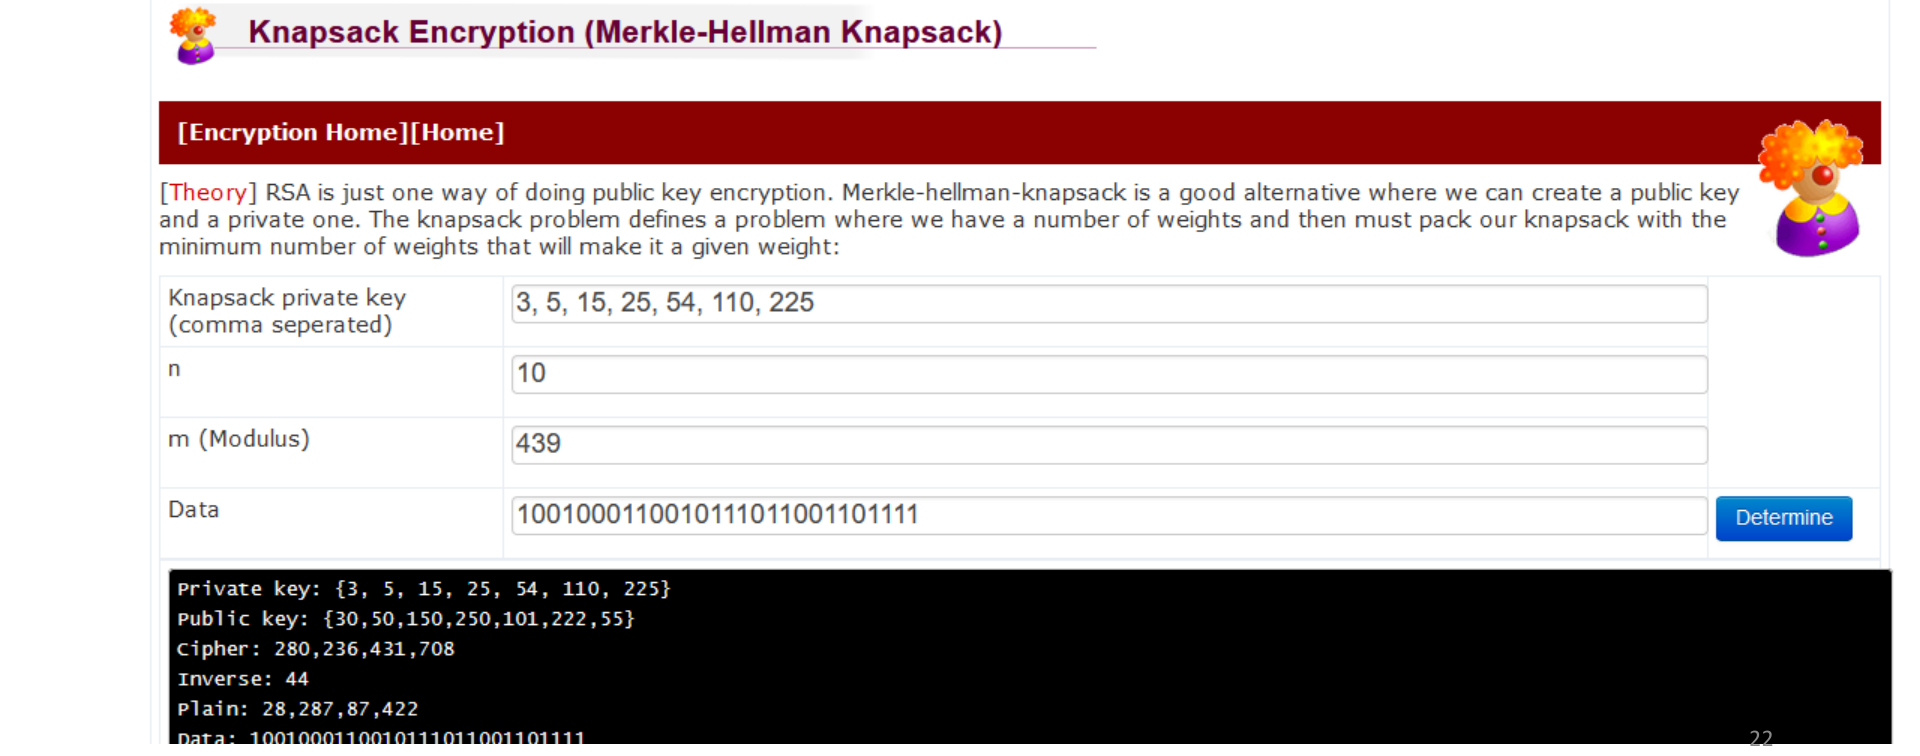
\includegraphics[width=\linewidth, height=0.45\textheight, keepaspectratio]{figures/demo-knapsack-online.png}
    \caption{Perkakas daring Merkle--Hellman yang dipakai pada
    Contoh~\ref{ex:demo-online}. Keluarannya mencetak kunci privat, kunci
    publik, kriptogram, invers, dan plainteks hasil dekripsi}
    \label{fig:demo-knapsack-online}
    \sumber{Munir, \textit{IF4020 Kriptografi}, ITB. Tangkapan layar perkakas
    daring.}
\end{figure}

\begin{obeactivity}
\textbf{Aktivitas 13.1: Simulasi Merkle-Hellman}
1. Tentukan kunci privat (barisan \textit{superincreasing}): $W_{priv} = \{2, 3,
   6, 13, 27, 52\}$.
2. Gunakan $m = 105$ dan $n = 31$. Periksa lebih dahulu bahwa $m > \sum_i w_i$
   dan bahwa $\text{PBB}(n, m) = 1$. Mengapa kedua syarat itu wajib?
3. Hitung kunci publik $W_{pub}$ menurut Persamaan~\eqref{eq:mh-kunci}.
4. Bandingkan $W_{priv}$ dengan $W_{pub}$. Tunjukkan dengan memeriksa setiap
   elemennya bahwa $W_{pub}$ bukan lagi barisan superincreasing.
5. Hitung $n^{-1} \bmod 105$.
\end{obeactivity}

Dua perkakas pada Listing~\ref{lst:knapsack-kunci} menjalankan langkah 3 dan 5
di atas: memotong rangkaian bit menjadi blok sepanjang $n$ bit, dan menghitung
barisan publik dari barisan privat.

\lstinputlisting[
    language=Python,
    caption={Pemotongan blok dan pembangkitan barisan publik Merkle-Hellman},
    label={lst:knapsack-kunci},
    firstline=113,
    lastline=123
]{\codefile{python/knapsack_uji.py}}

\begin{obeactivity}
\textbf{Aktivitas 13.2: Dekripsi \textit{Greedy} pada Barisan Superincreasing}
1. Periksa bahwa barisan $\{2, 3, 6, 13, 27, 52\}$ memenuhi
   Persamaan~\eqref{eq:superincreasing} untuk setiap elemennya.
2. Jalankan fungsi pada Listing~\ref{lst:knapsack-greedy} untuk memecahkan
   $M = 70$.
3. Tuliskan langkah demi langkahnya seperti pada
   Tabel~\ref{tab:greedy-70}, dan bandingkan hasilnya dengan
   Contoh~\ref{ex:greedy-superincreasing}.
4. Ubah $M$ menjadi $71$ dan jalankan kembali fungsinya. Mengapa fungsi itu
   mengembalikan \emph{tidak ada solusi}, dan apa artinya bagi keamanan pesan?
5. Ulangi untuk $M = 103$ (jumlah seluruh elemen). Bit apa yang dihasilkan?
\end{obeactivity}

\lstinputlisting[
    language=Python,
    caption={Pemeriksaan barisan superincreasing dan dekripsi \textit{greedy}},
    label={lst:knapsack-greedy},
    firstline=64,
    lastline=82
]{\codefile{python/knapsack_uji.py}}

\begin{obeactivity}
\textbf{Aktivitas 13.3: Enkripsi dan Dekripsi Tiga Blok}
1. Jalankan program pada Listing~\ref{lst:knapsack-enkripsi}, yang mengenkripsi
   \code{011000110101101110} dengan $W_{pub} = \{62, 93, 81, 88, 102, 37\}$.
2. Periksa bahwa kriptogramnya $(174, 280, 333)$.
3. Perhatikan bahwa $280$ dan $333$ melampaui $m = 105$. Jelaskan mengapa hal
   itu tidak merusak dekripsi.
4. Hitung $C' = (C \cdot n^{-1}) \bmod 105$ untuk ketiga kriptogram, lalu
   pecahkan hasilnya dengan algoritma \textit{greedy} pada $W_{priv}$.
5. Bandingkan hasilnya dengan Tabel~\ref{tab:mh-105-dekripsi}. Apakah ketiga
   blok pulih tepat seperti semula?
\end{obeactivity}

\lstinputlisting[
    language=Python,
    caption={Enkripsi dan dekripsi tiga blok dengan $m = 105$ dan $n = 31$},
    label={lst:knapsack-enkripsi},
    firstline=186,
    lastline=207
]{\codefile{python/knapsack_uji.py}}

\begin{obeactivity}
\textbf{Aktivitas 13.4: Mengukur Kerapatan dan Memeriksa Parameter}
1. Hitung kerapatan barisan $\{62, 93, 81, 88, 102, 37\}$ dengan
   Persamaan~\eqref{eq:densitas-knapsack}.
2. Hitung kerapatan barisan Merkle--Hellman yang dianjurkan sumber: 100 elemen
   dengan elemen terbesar sekitar 299 bit.
3. Bandingkan kedua nilai itu dengan ambang $d < 0{,}645$
   (Lagarias--Odlyzko) dan $d < 0{,}9408$ (Coster dan kawan-kawan).
   Barisan manakah yang justru dapat diserang?
4. Periksa anjuran modulus pada sumber: bisakah $m$ sepanjang 100--200 bit
   melampaui jumlah 250 elemen yang masing-masing bernilai 200 bit ke atas?
5. Bangkitkan barisan superincreasing sebanyak 100 elemen mulai dari sekitar
   $2^{200}$ dan hitung panjang bit jumlahnya. Berapa panjang $m$ yang
   sesungguhnya diperlukan?
\end{obeactivity}

\lstinputlisting[
    language=Python,
    caption={Kerapatan barisan, biaya penelusuran, dan pemeriksaan parameter},
    label={lst:knapsack-kerapatan},
    firstline=242,
    lastline=289
]{\codefile{python/knapsack_uji.py}}

\begin{obeactivity}
\textbf{Aktivitas 13.5: Membalik Kunci Publik Menjadi Kunci Privat}
1. Jalankan program pada Listing~\ref{lst:knapsack-balik}.
2. Perhatikan bahwa mengalikan $W_{pub}$ dengan $n^{-1}$ modulo $m$
   mengembalikan $W_{priv}$ secara tepat.
3. Jelaskan mengapa langkah itu sama persis dengan langkah kedua pada prosedur
   dekripsi (Subbagian~\ref{subsec:bukti-knapsack}).
4. Sekarang pikirkan posisi penyerang. Bila ia mengetahui barisan publik tetapi
   bukan $(n, m)$, persoalan apa yang harus ia pecahkan? Berapa banyak pasangan
   $(n, m)$ yang mungkin, dan mengapa menelusuri seluruhnya tidak praktis?
5. Uraikan secara ringkas mengapa Shamir dapat menemukan $(n, m)$ itu dalam
   waktu polinomial, sedangkan penelusuran menyeluruh tidak mungkin
   (Subbagian~\ref{sec:kriptanalisis-knapsack}).
\end{obeactivity}

\lstinputlisting[
    language=Python,
    caption={Pemulihan kunci privat dari kunci publik},
    label={lst:knapsack-balik},
    firstline=292,
    lastline=303
]{\codefile{python/knapsack_uji.py}}

Seluruh sepuluh pengujian pada program ini dapat dijalankan sekaligus dengan
\texttt{python knapsack\_uji.py}. Bila setiap angka pada bab ini cocok, program
akan mencetak \texttt{LULUS} pada setiap blok pengujian.


\begin{obereflection}
\textbf{Latihan 13.1}
1. Mengapa jumlah elemen di dalam barisan \textit{superincreasing} harus cukup besar untuk keamanan praktis?
2. Apa yang terjadi jika $\text{PBB}(n, m) \neq 1$ dalam proses pembangkitan kunci?
3. Jelaskan mengapa algoritma \textit{greedy} hanya bekerja pada barisan \textit{superincreasing} dan gagal pada barisan normal.
\end{obereflection}

\section{Rangkuman}
\begin{itemize}
    \item Persoalan \textit{knapsack} mencari bit $b_i \in \{0,1\}$ dengan $\sum_i b_i w_i = M$; versi umumnya tergolong \textbf{NP-complete} sehingga menjadi dasar awal keamanan sistem Merkle--Hellman.
    \item Barisan \textit{superincreasing} memenuhi $w_i > \sum_{j<i} w_j$, sehingga solusinya dapat ditemukan secara \textit{greedy} dalam waktu linier $O(n)$.
    \item Merkle--Hellman menyembunyikan barisan \textit{superincreasing} $W_{priv}$ menjadi kunci publik $w'_i = (w_i \cdot n) \bmod m$, dengan syarat $m > \sum_i w_i$ dan $\text{PBB}(n,m)=1$.
    \item Enkripsi menjumlahkan elemen publik yang bitnya $1$, $C = \sum_i b_i w'_i$, dan menghasilkan satu kriptogram bilangan bulat per blok.
    \item Dekripsi menghitung $C' = (C \cdot n^{-1}) \bmod m$ lalu memecahkan $C'$ dengan algoritma \textit{greedy} atas $W_{priv}$.
    \item Keamanannya patah: Shamir (1982) merekonstruksi barisan \textit{superincreasing} dari kunci publik dalam waktu polinomial, sehingga algoritma ini tidak dipakai secara praktis.
    \item Meski demikian, Knapsack berperan penting secara historis sebagai salah satu sistem kunci-publik pertama dan pendorong lahirnya konsep kriptografi kunci-publik.
\end{itemize}


\begin{obeassessment}
\textbf{Kuis Bab 13}
1. Apa perbedaan antara \textit{NP-complete problem} dan persoalan yang dapat diselesaikan dalam waktu polinomial?
2. Jelaskan langkah-langkah transformasi dari kunci privat ke kunci publik pada sistem Merkle-Hellman.
3. Mengapa penemuan Adi Shamir membuat algoritma Knapsack tidak lagi aman?
\end{obeassessment}
\begin{competencychecklist}
\begin{tabularx}{\linewidth}{|X|c|}
\hline
Indikator Kompetensi & Tercapai \\
\hline
Saya dapat menjelaskan konsep \textit{Knapsack Problem} & [ ] \\
\hline
Saya dapat membedakan barisan \textit{superincreasing} dan normal & [ ] \\
\hline
Saya dapat menghitung enkripsi sistem Merkle-Hellman & [ ] \\
\hline
Saya dapat melakukan dekripsi dengan bantuan invers modulo & [ ] \\
\hline
Saya dapat menganalisis penyebab kegagalan keamanan algoritma Knapsack & [ ] \\
\hline
\end{tabularx}
\end{competencychecklist}


\end{document}
